%%%%%%%%%%%%%%%%%%%%%%%%%%%%%%%%%%%%%%%%%

\chapter{Ultracold neutrons}\label{chap:UCN}

%%%%%%%%%%%%%%%%%%%%%%%%%%%%%%%%%%%%%%%%%

Ultracold neutron(s) (\ucn) are neutrons of very low kinetic energy ($\lesssim$\qty{300}{\nano\eV}) and have a number of very convenient properties that make them useful in experiments involving fundamental physics. Modern nEDM experiments are performed almost exclusively using UCN \cite{BAK06, SER15, ABE20} (an alternative is proposed in Ref.~\cite{PIE13}). Depending on the optical potential, \ucn may be contained at all angles of incidence by material bottles (Sec.~\ref{sec:ucn_matter_int}). They are also of low enough energies that they may be influenced by gravitational and magnetic potentials (Sec.~\ref{sec:ucn_grav_em}). Due to the ease of manipulation and transport, \ucn can be moved away from the production source, where backgrounds are typically high, into shielded environments where backgrounds may be controlled. \ucn are easy to polarize, and their polarization is easily measured (Sec.~\ref{sec:ucn_polarizers}). Neutrons are also abundantly available (albeit bound in nuclei) and when freed have a long lifetime (Sec.~\ref{sec:weak_interaction}).

%%%%%%%%%%%%%%%%%%%%%%%%%%%%%%%%%%%%%%%%%

\section{UCN properties}

%%%%%%%%%%%%%%%%%%%%%%%%%%%%%%%%%%%%%%%%%

A population of \ucn may be treated as an ideal gas with a few unique characteristics \cite{golubUCN}: 
%
\begin{itemize}
    \item \ucn wall collisions are mostly elastic and specular. Inelastic scattering results in a neutron being upscattered (heated) from the \ucn energy range and lost. \ucn gas in a container is a pseudo equilibrium where the gas velocity space is isotropic in the storage volume
    \item UCN\textendash UCN collisions are negligible, and the mean free path of a \ucn is characterized by the geometry of the storage volume
    \item Due to gravity, \ucn density tends to decrease as height increases within the storage volume.
    \item \ucn gas density decreases over time as \ucn are lost to $\beta$ decay and wall collisions.
\end{itemize}
%
\ucn flow in guide tubes is similar to rarified gas flow in tubes, with the same caveats described above.

%%%%%%%%%%%%%%%%%%%%%%%%%%%%%%%%%%%%%%%%%

\section{Gravitational and electromagnetic interactions}\label{sec:ucn_grav_em}

%%%%%%%%%%%%%%%%%%%%%%%%%%%%%%%%%%%%%%%%%

\ucn are of sufficiently low energy such that the influence of gravity is non-negligible. For gravitational acceleration $g_0$ acting on a neutron mass \gls{m_n}, the potential energy of at a height $h$ is given by
%
\begin{gather}
    V_g = \gls{mg}h
\end{gather}
%
where $\gls*{mg}=$\glsvalue*{mg} \cite{codata_2018}.

The magnetic moment of the neutron also interacts with a magnetic field \gls*{bField}, with the potential energy defined by
%
\begin{gather}
    V_m = - \vv{\gls{mu_n}}\cdot \gls*{bField}
\end{gather}
%
where $\gls*{mu_n}=60.307\,739(15)\text{ neV T}^{-1}$~\cite{codata_2018}. Spin dependent interactions in a magnetic field are further described in Chap.~\ref{chap:spinManipulation}.

The neutron charge limit is effectively zero~\cite{baumann_neutron_charge}
%
\begin{gather}
    \gls*{q_n}=\glsvalue*{q_n}\quad(68 \% \text{ c.l.})
\end{gather}
%
Due to the internal charge distribution of the neutron quark structure, a neutron subjected to an external electric field creates an induced EDM given by $d_\text{induced}=4\pi \epsilon_0 \alpha_\text{n} E$. The neutron polarizability $\alpha_\text{n}$ is $(11.8\pm 1.1)\,10^{-4}\text{ fm}^3$~\cite{pdg2022}, giving $d_\text{induced}\sim 10^{-32}e\,\text{cm}$. This is well below the sensitivity of the \acrshort*{lanl} \acrshort*{nedm} experiment.


%%%%%%%%%%%%%%%%%%%%%%%%%%%%%%%%%%%%%%%%%

\section{Weak interaction}\label{sec:weak_interaction}

%%%%%%%%%%%%%%%%%%%%%%%%%%%%%%%%%%%%%%%%%

\begin{figure}[htp]
    \centering
    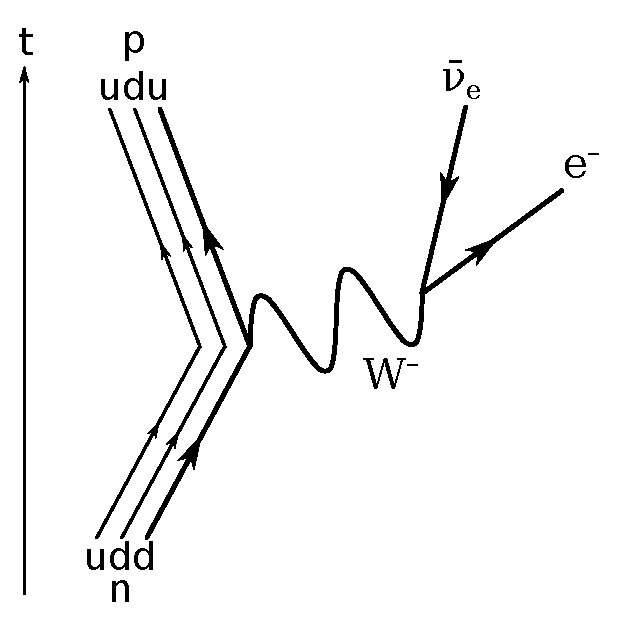
\includegraphics[width=0.3 \textwidth]{figures/beta_negative_decay.pdf}
    \caption[Feynman diagram of free neutron $\beta$ decay]
    {Feynman diagram of free neutron $\beta$ decay. Image from \cite{beta_decay_fig}}
    \label{fig:beta_decay}
\end{figure}

Free neutrons undergo $\beta$ decay
%
\begin{gather}
    \text{n}\rightarrow \text{p}+ e^-+\bar{\nu}_e
\end{gather}
%
governed by the neutron lifetime (decay time) $\gls{tau_n}=\glsvalue*{tau_n}$ \cite{pdg2022}. The Feynman diagram for this process is given in Fig.~\ref{fig:beta_decay}. The neutron lifetime designates the amount of helium created during Big Bang nucleosynthesis. The CKM matrix element $V_\text{ud}$ (Eq.~\ref{eq:CKM}) can also be determined from measurements of \gls{tau_n} in combination with measurements of $0^+\rightarrow0^+$ decays \cite{Young2014}.

The most accurate neutron lifetime experiments to date have been storage experiments with \ucn held by magnetic and gravitational potentials, such as the UCN$\tau$ experiment at \acrshort{lanl} \cite{gonzalez_ucn_tau}. There is an ongoing disagreement between neutron lifetime storage experiments that count surviving \ucn and neutron lifetime cold beam experiments that count the proton decay products~\cite{czarnecki2018}.

The neutron beta decay directional distribution and total decay rate can be very generally written in terms of the neutron spin and lepton momenta \cite{Young2014}
%
\begin{align}
    d\Gamma(\vv{p}_e, \vv{p}_{\bar{\nu}}) &= dE_e\,d\Omega_e \,d\Omega_{\bar{\nu}} \frac{F(E_e)\,p_e E_e (E_o-E_e)^2}{(2\pi)^5} \xi \nonumber \\
    &\quad\quad \times \left[1 + a\frac{\vv{p}_e \cdot \vv{p}_{\bar{\nu}}}{E_e E_{\bar{\nu}}}
    +b\frac{m_e}{E_e} + \langle \vv{S}_\text{n} \rangle \cdot
    \left( A\frac{\vv{p}_e}{E_e} + B \frac{\vv{p}_{\bar{\nu}}}{E_e} + D\frac{\vv{p}_e\times \vv{p}_{\bar{\nu}}}{E_e E_{\bar{\nu}}}
    \right) \right]
\end{align}
%
$\vv{S}_\text{n}$ is neutron spin, $F(E_e)$ is the Fermi function for final state interactions, $E_o$ is the endpoint energy, $E_e$ and $\vv{p}_e$ are electron energy and momentum, and $E_{\bar{\nu}}$ and $\vv{p}_{\bar{\nu}}$ are anti-neutrino energy and momentum.

Of interest are correlation coefficients $a$, $b$, $A$, $B$, and $D$, which are experimental observables. Measurements of these coefficients are a probe of the V\textendash A structure of the \acrshort*{sm}. 
%
\begin{itemize}
    \item Electron-antineutrino asymmetry $a$ is measured from the proton spectrum.
    \item Fierz interference coefficient $b$ is measured from the $\beta$ spectrum. $b$ is nominally $0$ in the \acrshort*{sm}.
    \item Beta asymmetry $A$ is determined from the angular correlation between the emitted electron and neutron polarization.
    \item Spin-antineutrino asymmetry $B$ is found via the angular correlation of the recoil proton and neutron polarization.
    \item Triple product $D$ arises from the triple correlation between electron momentum, proton momentum, and neutron spin. $D$ is also nominally $0$ in the \acrshort*{sm}.
\end{itemize}

Reference~\cite{Young2014} provides a review of the $\beta$ decay experimental program at \acrshort{lanl}. (In this section we followed conventional notation for $\beta$ decay observables, but variables $a$, $b$, $A$, $B$, and $D$ will be used to denote other parameters for the remainder of this dissertation.) 


%%%%%%%%%%%%%%%%%%%%%%%%%%%%%%%%%%%%%%%%%

\section{Strong interaction}

%%%%%%%%%%%%%%%%%%%%%%%%%%%%%%%%%%%%%%%%%

Neutrons and protons are bound in nuclei via the strong interaction. In the low energy limit the strong force between the proton and neutron can be approximated by attractive square-well potential of depth \qty{40}{\mega\eV} with radius $2\times10^{-5}\text{ m}$. A more accurate representation is the Fermi potential, a square well with rounded corners. This Fermi potential is not to be confused with the optical potential (also proposed by Fermi) described in Sec.~\ref{sec:ucn_matter_int}. The force between a neutron and a nucleus is also approximated by a square well with $r=r_0A_m^{1/3}$ for mass number $A_m$ and the constant $r_0=1.2\times10^{-15}\text{ m}$ \cite{golubUCN}.

Neutrons may be absorbed (captured) by nuclei. When absorbed, a $\gamma$ ray or charged particle ($[\text{n},\text{p}]$ or $[\text{n},\alpha]$) is released. Absorption cross sections are further discussed in Sec.~\ref{sec:ucn_absorption}.

%%%%%%%%%%%%%%%%%%%%%%%%%%%%%%%%%%%%%%%%%

\section{UCN interactions with matter}\label{sec:ucn_matter_int}

%%%%%%%%%%%%%%%%%%%%%%%%%%%%%%%%%%%%%%%%%

Chapter 2 of Ref.~\cite{golubUCN} provides a very thorough description of neutron interactions with matter. The interaction of a \ucn with some material is given by a complex optical potential, or pseudo-potential, of the form
%
\begin{gather}
    U = V - iW = \frac{2\pi\hbar^2}{\gls{m_n}}\gls*{rho_N} b_c-i\frac{\hbar}{2}\gls*{rho_N} \sigma_\ell v \label{eq:optical_potential}
\end{gather}
%
where \gls{m_n} is the neutron mass, $v$ is the velocity of the neutron, $b_c$ is the coherent neutron scattering length of the material, $\sigma_\ell$ is the loss cross section, and $\gls*{rho_N}$ is number density. Number density can be expressed in units~[\unit{\meter^{-3}}] by the relation $\gls*{rho_N}=\rho_\text{mat}N_A/w_\text{at}$, where $\rho_\text{mat}$ [\unit{\g\per\m^3}] is material density, $w_\text{at}$ [\unit{\g\per\mole}] is atomic weight, and $N_A$ [\unit{\mole^{-1}}] is Avogadro's number.

The real component of optical potential $V$ describes the critical neutron energy that may be confined by a material (Sec~\ref{sec:ucn_transmission} and \ref{sec:ucn_reflection}), and the imaginary part $W$ describes absorption and upscattering (Sec~\ref{sec:ucn_absorption} and \ref{sec:ucn_reflection}). Table~\ref{tb:optical_potentials} lists the UCN optical potentials of commonly used materials in the LANL nEDM experiment.

\begin{table}[bp]
\centering
\caption[UCN optical potentials of selected materials. V is the real component and W is the imaginary component]{\label{tb:optical_potentials}UCN optical potentials of selected materials. $V$ is the real component and $W$ is the imaginary component.}
\begin{tabular}{
    l
    S
    S[exponent-mode = scientific, table-format = 2.2e1]
    l
}
\toprule
Material & {V [\unit{\nano\eV}]} & {W [\unit{\nano\eV}]} & Ref.\\ 
\midrule
Al & 54.1 & 0.00281 & \cite{atchison_transmission_2009}\\
Cu & 170.747 & 0.0726 & \\
\bottomrule
\end{tabular}
\end{table}

%%%%%%%%%%%%%%%%%%%%%%%%%%%%%%%%%%%%%%%%%

\subsection{Transmission}\label{sec:ucn_transmission}

%%%%%%%%%%%%%%%%%%%%%%%%%%%%%%%%%%%%%%%%%


%%%%%%%%%%%%%%%%%%%%%%%%%%%%%%%%%%%%%%%%%

\subsection{Absorption}\label{sec:ucn_absorption}

%%%%%%%%%%%%%%%%%%%%%%%%%%%%%%%%%%%%%%%%%

The absorption cross section $\sigma_\text{abs}$ is proportional to $1/v$

%%%%%%%%%%%%%%%%%%%%%%%%%%%%%%%%%%%%%%%%%

\subsection{Reflection}\label{sec:ucn_reflection}

%%%%%%%%%%%%%%%%%%%%%%%%%%%%%%%%%%%%%%%%%

\comment{Loss per bounce. Blue book Eq. 2.70. Refer to Pattie et al 2017 Loss Factor vs LPB}

%%%%%%%%%%%%%%%%%%%%%%%%%%%%%%%%%%%%%%%%%

\subsection{Beer-Lambert Law}\label{sec:beer_lambert_law}

%%%%%%%%%%%%%%%%%%%%%%%%%%%%%%%%%%%%%%%%%

Neutron flux attenuation after passing through material may be described with the Beer-Lambert law. Here we demonstrate a way to model neutron absorption or scattering during transmission.

Let a beam of neutrons be incident on a material with area $A$, thickness $dx$, and density of atoms (number density) $\gls*{rho_N}$. The number of atoms hit by the incident beam of intensity $I$ is given by $\gls*{rho_N} A\,dx$. The ``effective area'' of the atoms is given by $\sigma \gls*{rho_N} A \, dx$, where $\sigma$ is an absorption or scattering cross section of neutrons on the material.

Therefore, the probability of the a neutron being absorbed or scattered out of the beam in a material of thickness $dx$ is given by
%
\begin{gather}
    -\frac{dI}{I}=\frac{\sigma\gls*{rho_N} A}{A}dx
\end{gather}
%
where $dI$ is the change in intensity as the beam traverses the distance $dx$. Integrating both sides of the equation gives
%
\begin{align}
    \int^I_{I_0}\frac{dI}{I} &= -\int^x_0 \sigma \gls*{rho_N} \,dx \\
    \ln \frac{I}{I_0} &= -\sigma \gls*{rho_N} x \\
    \frac{I}{I_0} &= e^{-\sigma \gls*{rho_N} x} \label{eq:beer_lambert_law_variant}
\end{align}
%
Where $I_0$ is the beam density intensity at the entrance of the material. Defining the mean free path inside the material as $\lambda_\text{mfp}=1/(\gls*{rho_N} \sigma)$ we get the Beer-Lambert law, which describes flux attenuation.
%
\begin{gather}
    I(x) = I_0 e^{-x/\lambda_\text{mfp}} \label{eq:beer_lambert_law}
\end{gather}
%
 The Beer-Lambert law applies to neutrons, photons, and rarefied gases. See Appx.~\ref{appx:199hg_pumping} for an example application to the \qty{254}{\nano\meter} laser used for optical pumping of the $\ce{^199Hg}$ comagnetometer. 
 
 The probability $P_\text{elastic}$ of bulk elastic scattering after traversing a distance $x$ through a material is given by
%
\begin{gather}
    P_\text{elastic}=1-e^{-x \gls*{rho_N} \sigma_\text{inc}}
\end{gather}
%
where $\sigma_\text{inc}$ is the incoherent cross section for thermal neutrons (see Ref.~\cite{nist_neutron_cross_sections}). Similarly, the chance for absorption in a material for a \ucn with velocity $v$ may be described by
%
\begin{gather}
    P_\text{abs}= 1-e^{-x \gls*{rho_N} \sigma_\text{abs}v_\text{thermal}/v}
\end{gather}
%
where $\sigma_\text{abs}$ is the absorption cross section for thermal neutrons ($v_\text{thermal}=\qty{2200}{\meter\per \s}$) as listed in Ref.~\cite{nist_neutron_cross_sections}.
